%!TEX root = ../template.tex
%%%%%%%%%%%%%%%%%%%%%%%%%%%%%%%%%%%%%%%%%%%%%%%%%%%%%%%%%%%%%%%%%%%%
%% chapter2.tex
%% NOVA thesis document file
%%
%% Chapter with the template manual
%%%%%%%%%%%%%%%%%%%%%%%%%%%%%%%%%%%%%%%%%%%%%%%%%%%%%%%%%%%%%%%%%%%%

\typeout{NT FILE chapter2.tex}

% \printbibliography[heading=subbibliography, segment=\therefsegment, title={\bibname\ for chapter~\thechapter}]
\glsresetall
\chapter{State of the Art}\label{cha:II_SotA}
% escrever aqui qlq coisa de introduçao:

Like any project development, it is always a wise approach studying all the theoretical concepts and current state of the art beforehand. That's the objective of this Chapter; starting with the clarification of the intricate arrangement of satellites that constitute a GNSS in section~\ref{sec:}, the different positioning techniques inevitably become easier to disect, through sections~\ref{sec:}, \ref{sec:} and \ref{sec:}, as the explanation  the navigational methods in section~\ref{sec:}

Finally, the current most relevant solutions are addressed and compared, as these will provide helpful guidelines to the development of future beRTK.

% enter a NUTSHELL setting of RTK,
a base station is intended that is capable of fine-tuning the position of the rover (drone);

beRTK can be used for:
Enhanced Landing
Surveying fields precisely
Accurate Mapping
Review Work Processes

HEIFU, beRTK and beXStream can be used for:
    1. \textbf{Cartografy and 3D Mapping} -- Few years ago, the only way to get an aerial photogrammetric map of high accuracy and resolution was to fly the area of interest with a manned aircraft—or have access to a spy satellite. Those options are all costly and require recruiting people with specific skill sets.
    The advancements in drone capabilities such as 3D mapping software and their decreasing costs have made high quality aerial maps available for a multitude of people and number of sectors including construction, agriculture, mining, infrastructure inspection and real estate. Having a clear, accurate photograph or 3D model of your project area, complete with measurements, is advantageous in terms of decision-making.  
    Mapping with drones is done using a technique called Photogrammetry -- a science of making measurements from Photographs. The output of this is normally a map, measurement or 3D model of a real-world object or scene. Due to its capability to fly at a low altitude, it can capture high quality images. 

    2. \textbf{Detection and Removal of Asian Wasp hives} -- Asian Wasp Hives are created by various species such as the Asian Hornet that are indigenous to Southeast Asia.  Their presence can now be seen as a global phenomena, and it is vital that we continually innovate state of art solutions to tackle the spread. A single sting from this species, or even multiple stings at a time, can be fatal to people who are allergic to their venom.
    Modern technologies, such as the use of drones, can be used to detect the Asian wasp hives using its on-board video camera and destroy them via its inbuilt spraying mechanism.
    The drone aims to make the process of locating and destroying the hornets' nests not only faster and easier, but less environmentally aggressive. This process can be time-consuming and dangerous for humans, as it often involves using poles or ladders to reach nests on roofs or in treetops.

    3. \textbf{Precision Farming} -- Precision agriculture is a farming management concept based on observing, measuring, and responding to inter and intra-field variability in crops. It has been enabled by the advent of Global Navigation Satellite System (GNSS). Drones can monitor crops much more accurately, frequently, and affordably, delivering higher quality data that is updated regularly to provide insight into crop development and highlight inefficient or ineffective practices. This can help farmers decide when to plant and harvest crops.
    As a result, precision farming using drone technology through the collection of aerial maps of plantations can improve time management, reduce water and chemical use. This produces healthier crops and higher yields—all of which benefit farmers' production and conserve resources while reducing chemical runoff. It can also help agricultural producers to have a notion -- in real-time -- about the status of their plantations in specific areas and receive notifications about those that require more attention.
        a. Survey every inch of your field
        Allows detailed survey of every field
        b. Improves productivity and efficiency 
        Reduce time spent on field-walking
        c. Higher resolution of the field areas of interest 
        It is beneficial for immediate identification and GPS tagging
        d. Earlier identification of potential crop issues
        Use of multispectral sensing technology

    4. \textbf{Search and Rescue} -- Drone advancements in recent years have resulted in an increased capacity for unmanned vehicles to take on a range of dangerous tasks in emergency response that would traditionally have been performed by humans.
    They are flying to the rescue in the emergency response sector, helping police record and analyze crime scenes, and assisting search and rescue teams in identifying victims lost in the wilderness.
    The drone collects precise, detailed footage and data from the air, it can also help crews cut down on expenses, keep workers safe, and it can provide crews with footage that gives them an aerial advantage, without having to spend resources on expensive manned aerial flights. 

    5. \textbf{Forest Firing Detection and Monitoring} -- Having a fast and effective detection is a key factor is wildfire fighting. Over the years, efforts are made to focus on early response, accurate results in both daytime and nighttime and the ability to prioritise fire danger.
    Satellite and aerial monitoring through the use of UAVs can provide a wider view to monitor very large, high risk areas. These more sophisticated systems employ GPS and aircraft-mounted with infrared or high-resolution visible cameras. They capture wind direction, high-resolution imaginary of smoke to identify and target wildfires.
    Drones allow firefighters accurate data. By using the real-time data, firefighters can determine where a fire will move next, assisting them in making swift decisions and draw up a strategic plan about movement and evacuation.
    The use of UAVs limits exposure and reduces risk to pilots and wildland firefighters. They are easily packable and able to fly in remote locations. 

    6. \textbf{Border Patrol Monitoring} -- Border surveillance is a 24/7 operation that can't afford downtime or periods of reduced readiness. It involves guarding against illegal immigration, smuggling and terrorism demands.
    The rapid advances in technology has led to UAS (unmanned aerial systems) to identify, tract and analyse moving objects from the air with the ability to deploy from anywhere day or night. They can operate in demanding environments that are vulnerable to bad weather conditions and they can fly at a much more efficient cost and require far less training to use.

    7. \textbf{Demining} -- Demining is a process of removing, deactivating, or safely detonating land mines in an area.
    More than 100 million mines are still active in the world today. They pose a deadly threat to local communities, cause fear, mutilate limbs, limit travel, force the abandonment of infrastructure and hamper socio-economic development.
    Use of AI allows drones to autonomously map, detect and detonate land mines, they are equipped with infrared cameras allow detection of mines much faster in contaminated areas by measuring differences in temperature. The drone can cover a large area in a much shorter time than deminers on the ground. This technology has the potential to save time and make the work of mine clearance experts safer.
    
    8. \textbf{Medical Delivery} -- Medical delivery involves supplying health care services to meet the health needs of a target population. Telecommunication drones are being used for diagnosis and treatment, perioperative evaluation, and tele-mentoring in remote areas.
    Drones have the potential to be reliable medical delivery platforms for microbiological and laboratory samples, pharmaceuticals, vaccines, emergency medical equipment. Drones could deliver medications and supplies to patients being cared for in the home instead of a hospital-based setting.
    The future will see more outpatient care and even home-based care that used to be delivered in the hospital. For many conditions, drone technology may make it easier and safer to provide this home-based care. When a provider rounds on a home patient, blood can be drawn and immediately sent by drone to the lab to be tested. Medications, antibiotics and treatments ordered by the provider may be delivered to the home by drone.

    9. \textbf{Infrastructure} -- In recent years, it has been reported that the construction industry struggles with a great deal of inefficiency. Large construction projects typically take 20\% longer than expected to complete and are up to 80\% over budget.
    The use of drones in the supervision of infrastructures can reduce work accidents by up to 91\%. The inspection of infrastructures -- in the construction or maintenance phase -- allows to increase the safety of the site and work operations (identifying intrusions by intruders and preventing accidents at work).
    The areal monitoring -- in real time -- of the developments of a construction, increases the efficiency in the decision making by those responsible for the construction. They can also be used to monitor areas across long distances, such as vegetation rows, roads and railroads. Even before the launch of many construction projects, a topographic survey of the site is required to get a good understanding of the environment in which the project will take place. DTMs and DSMs of a site generated with drone data can show possible drainage points, changes in elevation and other factors that can assist in selecting the best locations for building, digging or storing materials. 

    10. \textbf{High Rise Window Cleaning} -- The job of cleaning windows on tall buildings ranks as one of the most dangerous jobs in the world due to the amount of health and safety procedure required. The cost of infrastructure and labor resources tend to make this expensive.
    With the implementation of Window Cleaning drones, building maintenance will become more efficient and safer. Window Cleaning drones will ensure a safe work environment without ropes and scaffolding.
    With a drone, you can do this work without any set-up and dismantling extremely safely whereby each arm will have the capacity to water and clean the window in parallel. 
    
    11. \textbf{Ad hoc Communication Relay} -- Imagine when telecommunications infrastructure is damaged by natural disasters, or a remote area where there are no communication towers, creating a network that can handle voice channels can be vital for many purposes.
    Technological developments in Unmanned Aerial Vehicles (UAV) equipped with WIFI access points could be rapidly deployed to provide wireless coverage to ground users. This WIFI access network in turn can be used to provide a reliable communication service to ground users. 

    12. \textbf{Equipment Monituring in factories} -- As part of Maintenance procedures, every industry requires a visual inspection to be conducted. It involves a thorough review with the naked eye of every single part of an asset.
    Traditionally, when inspecting a cell phone tower, an inspector will climb the entire tower looking for areas that might need maintenance. For indoor inspections, such as those performed inside boilers or pressure vessels, inspectors must build scaffolding so they can climb up the sides of the boiler, visually reviewing every square inch as they go.
    Visual inspections are critical to ensuring the proper maintenance of a company's assets. Drones in inspection helps to eliminate time consuming and substantial risk activities.
    Some companies can prove that what once took maintenance workers up to 12 hours to complete by climbing on automated platforms and scaffolding is now said to be accomplished in 12 minutes. By using high-resolution cameras mounted on easily piloted drones, companies could benefit from eliminating risk to staff, increasing overall efficiency and garnering the same (if not more accurate) results. 

    13. \textbf{Remote Car Inspection - Insurance} -- Drones can become a valuable tool for the Automotive industry, it can aid the accuracy, speed and thoroughness of assessing the extent and cost of damage.
    We know how lengthy, manual, and cumbersome going through the assessment process can be. When a car is involved in an accident, the insurance company sends a car to a workshop and they have the capability to utilise drone technology to inspect and assess the car. Its capability to produce 3D images can be used to trigger other processes such as estimating cost of repairs.
    The drone would be controlled in distance through the application. A report is then produced compiling information that will help jump start and shorten the overall process of the repair. 
    
    14. \textbf{Virtual Traveling} -- Tourism is an activity that may be expensive, dangerous, and limited to people who are physically unable to visit certain landmarks.
    Virtual travelling allows people to travel without the hassle: no jet lag, no language barriers, no expensive price tags. Travel without breaking the bank, maybe even without leaving the house and exposing you to the danger. Most of all, it could help bring people to places that are otherwise inaccessible. The prospect to explore any part of the world from one's own home is a classic sci-fi dream. 
    This is the new way to explore the world we live in, giving the opportunity to visit every dream destination in the comfort of your home or even provide a travel safeness like no other. Virtual Travelling seems tailor-made for such individuals, providing the freedom to explore without the stress of ensuring safe access.     
    By purchasing our UAVs and its extras, you will be able to provide unique experiences to people with a real-time experience without them leaving the comfort of their sweet home. Now its easy to provide people the visit to their dream destination or even to their favourite country.  

% |=|=|=|=|=|=|=|=|=|
But there is still a great ally for such efficiency, which sometimes goes unnoticed is even forgotten: Image Processing.

Começar com:
I. o que é uma base station? fazer analogia
II. dizer para que e que serve
III. onde/no que é que eu vou empregá-la?
IV. que tecnologias utiliza?
V. explicar cada tecnologia relativamente a base

Talk about:
    1. Satellite Navigation Device
    2. Transceiver
    3. Base station
    4. Aerial base station
    5. how GPS works - https://electronics.howstuffworks.com/gadgets/travel/gps.htm
    6. how satellites work - https://science.howstuffworks.com/satellite.htm
    7. atomic clocks - https://science.howstuffworks.com/atomic-clock.htm

    8. differential GPS (DGPS) - The term differential GPS, or DGPS, sometimes indicates the application of this technique with coded pseudorange measurements
    8.1. relative GPS - usually indicates the application of this technique with carrier phase measurements
    8.2. carrier phase measurements
    8.3. baselines
    in: https://www.e-education.psu.edu/geog862/node/1725

    9. GNSS - The performance of GNSS is assessed using four criteria: Accuracy, Integrity, Continuity and Availability. The correlated range errors due to ephemeris prediction errors and residual satellite clock, ionosphere and troposphere errors may vary slowly with time and user location.
    Therefore, by comparing pseudo-range measurements with those made by equipment at a presurveyed location, known as a REFERENCE STATION or BASE STATION, the correlated range errors may be calibrated out, improving the navigation-solution Accuracy! This is the priciple behind Differential GNSS (DGNSS)~\cite{edseee_9101092}. % fazer desenho .svg de base station a "acertar" o drone com os satelites
    10. L2C and L5 (signal availability) bands;
    11. the future L1C
    12. Capacity of continuous measurements
    13. static precision measurement
    14. dynamic precision measurement
    15. what is a 120-channel receiver?
    16. explicar o que cada célula do excel significa, tanto as que considerei mais importantes como as outras
    17. RTK / RTK-GNSS / D-RTK / dynamic differential technology~\cite{ayers_geosystems_2011}
       
    land surveying - In the context of external land surveying, a base station is a GPS receiver at an accurately-known fixed location which is used to derive correction information for nearby portable GPS receivers. This correction data allows propagation and other effects to be corrected out of the position data obtained by the mobile stations, which gives greatly increased location precision and accuracy over the results obtained by uncorrected GPS receivers.

    how long does it take for a radio signal to be emitted from a satellite to reach the surface of the earth? 
    R.: given that a satellite circles the globe at an altitude of about 19.3 km --> d = v*t => 19.3*10$^3$ / 300 000 000 = t = 6.43*10$^{-5}$ = 64.3 us.

% artigos que li:
a. Experimental Testbed and Methodology for the
Assessment of RTK GNSS Receivers Used
in Precision Agriculture;

b. DETERMINATION OF THE POSITION USING
RECEIVERS INSTALLED IN UAV

c. High-Precision/Throughput Growth Measurement of
Crops by Drone with Stereo Matching Based on
RTK-GNSS and Single Camera

d. Estimation of the Base Station Position Error in a
RTK Receiver Using State Augmentation in a
Kalman Filter

e. Resilient Deployment of Drone Base Stations

f. Based on a single-base station RTK control survey
and precision analysis 

g. Design of an Autonomous drone for IoT deployment
analysis 

h. RTK+ System for Precise Navigation in Shadowed
Areas 




\section{Global Navigation Satellite System}\label{II_gnss}

%MUDAR, ESTÁ COPIADO!
So, the difference between RTK and DGPS is that DGPS is the traditional differential GPS.
RTK is a specific type of DGPS.
but it uses a newer technology than the traditional DGPS.
RTK stands for real-time kinematic and commonly uses the RTCM protocol.
The traditional DGPS uses an older antiquated protocol while RTK uses a newer algorithm, and the protocol is based on RTCM3. 
%____________

Nowadays, whenever someone wishes to know their current location on Earth, just a few, effortless taps on a smartphone will be enough; this is often associated with GPS, which has been around for many years. In a more general manner, this technology can be described as a Global Navigation Satellite System, or GNSS. This term refers to any satellite constellation that can be used to help navigate throughout the world (as the name suggests). derives from a set of artificial satellites that comprises a network, and such network belongs 

to the average smartphone nowadays works as a GNSS receiver.
global navigation satellite system comprises a network of satellites that continuously orbit the Earth, constantly emmiting radio-frequecy (hyphen?) signals carrying information about their current status, position in space and precise time.
This information is acheived through atomic clocks, installed within the satellite itself.

smartphone = single-band ou multi-band?
how many constellations;
how many satellites in each constellation;
% falar de todos os topicos que estejam no doc Word GNSS

\section{RTK}\label{II_rtk}
% falar de todos os topicos que estejam no doc Word RTK (single- multi-link,...)
% link da base station ao UAV

\section{NTRIP}\label{sec:II_ntrip}
% falar de todos os topicos que estejam no doc Word NTRIP

\section{Battery System}\label{sec:II_battery}
% falar de todos os topicos que estejam no doc Word Battery

The formula is (Wh)/(h) = (W). For example, if you have 100 Wh for a duration of 2 hours, then the wattage is (100)/(2) = (50) Watts.
(Watthours is a measure of energy and watts is a unit of power. Power multiplied by time is enery).

como cada uma das baterias atualmente em uso is rated for (as?) 7.4V, 1070 mAh, that corresponds to 7.918 Wh.

% LiFePO$_4$ better than Li-ion batteries?
``The LiFePO$_4$ battery has the edge over lithium-ion, both in terms of cycle life (it lasts 4-5x longer), and safety. This is a key advantage because lithium ion batteries can overheat and even catch fire, while LiFePO4 does not''% citation needed

\subsection{USB Type-C}\label{sec:II_usb_c}
% ler wiki do USB-C e derivar os topicos daí
% depois ir ao IEEEXplore procurar papers que dêem backup
\subsubsection{Power Delivery}\label{sec:II_usb_c_PD}
% PD is a protocol

\section{Current Solutions}\label{sec:II_curr_solutions}

% \begin{tabularx}

% \end{tabularx}

\begin{table}[ht]       % provavelmente devo meter as palavras "parameter"/"base station" na caption?
	\centering          % ou devo eliminar a celula toda?
    \captionsetup{justification=centering}
    \caption{Compilation of the most relevant solutions available in the market (as of the date of the present document).}
	\label{tab:current_solutions_1}
	\begin{tabular}{|c|c|c|c|c|c|} % 8 colunas
		\toprule
		
        {} & {} & {} & \vtop{\hbox{\strut \textbf{beRTK}}\hbox{\strut \textbf{(Beyond Vision)}}} & \vtop{\hbox{\strut \textbf{Reach RS2}}\hbox{\strut \textbf{(Emlid)}}} & \vtop{\hbox{\strut \textbf{D-RTK 2}}\hbox{\strut \textbf{(DJI)}}}\\        
        
        \midrule

        \multirow{8}{*}{\rotatebox{90}{\textbf{Positioning}}}&\textbf{CorrectionT}\\
        &\multirow{5}{*}{\rotatebox{90}{\textbf{SupportedC}}}&\textbf{GPS}\\
        &\textbf{GLONASS}\\
        &X\\
        &X\\
        &X\\
        &X\\
        &X\\
        \midrule
        
        \rotatebox{90}{\textbf{Connectivity}} & 2 & 2 & 2 & 2 & 2\\
        \midrule

        \multirow{2}{*}{Multirow}&X\\
        &X & t\\

        \midrule\addlinespace[1.5ex]
        
        {} & 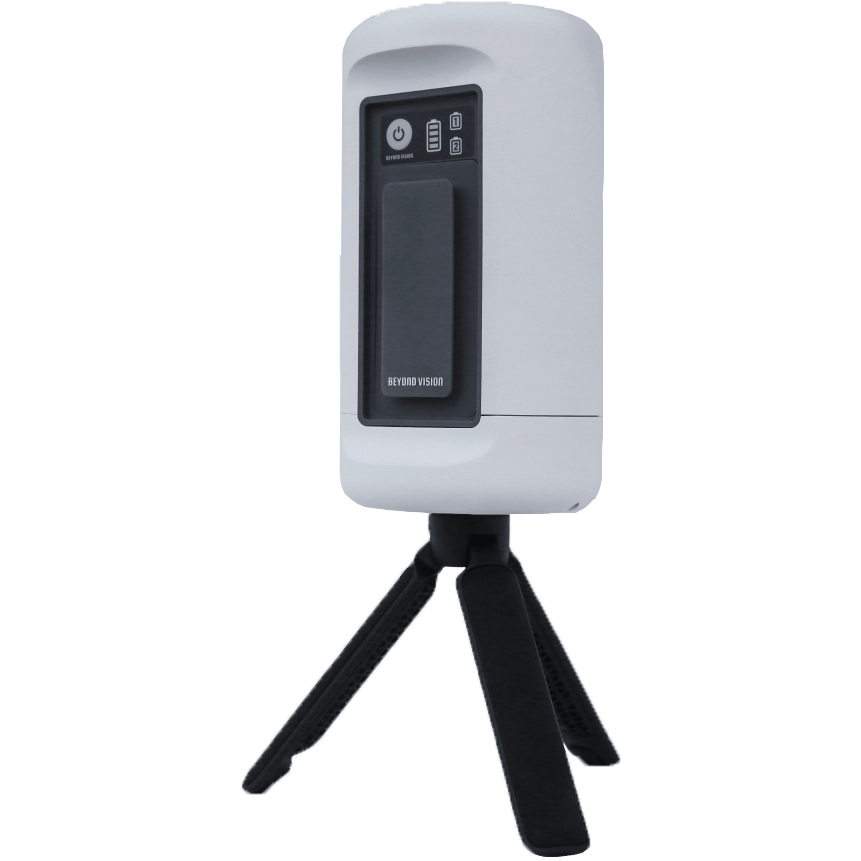
\includegraphics[height=1.4cm]{Chapters/Figures/base_stations/beRTK_2.png} & 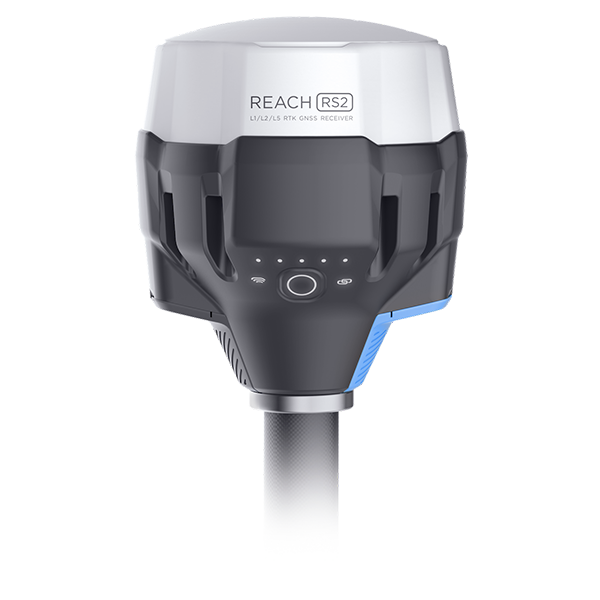
\includegraphics[height=1.4cm]{Chapters/Figures/base_stations/REACH-RS2.png} & 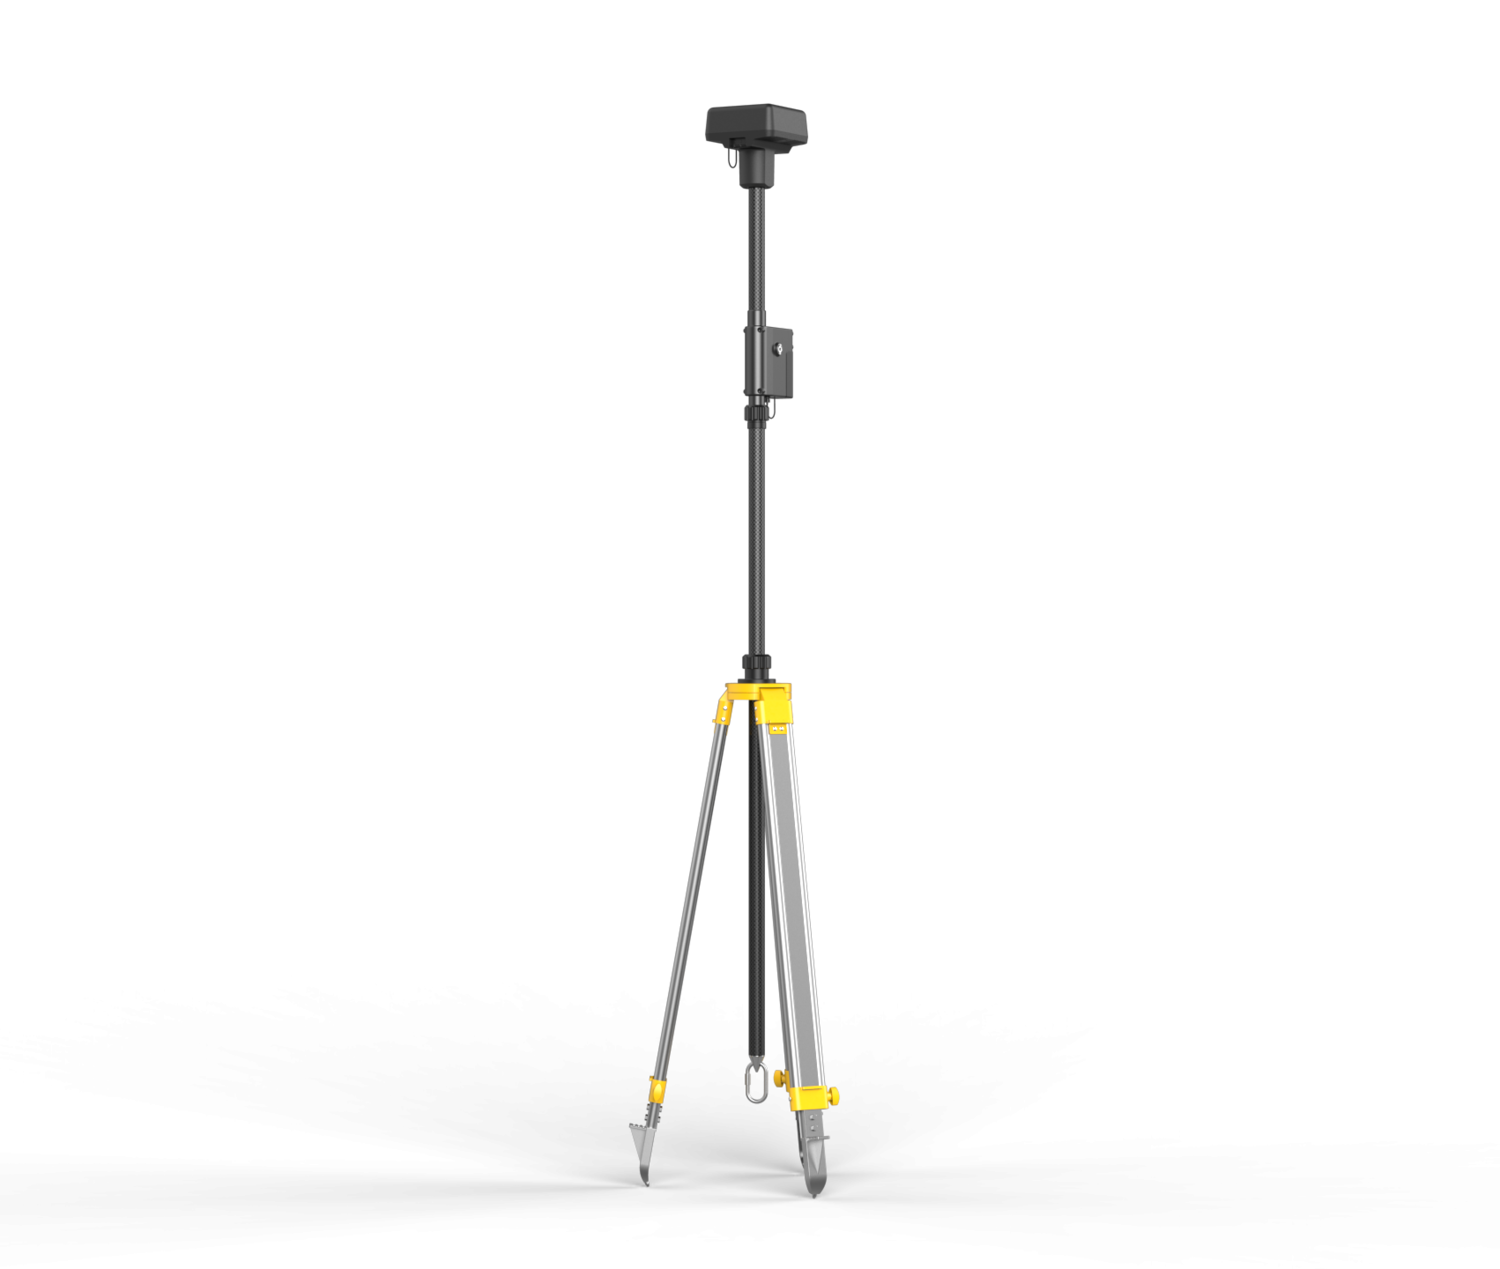
\includegraphics[height=1.4cm]{Chapters/Figures/base_stations/d-rtk-2.png}\\
		
        \bottomrule
        
	\end{tabular}
\end{table}

% tabela como multirow dento de multirow:
% \multirow{6}{*}{W2} & \multirow{3}{*}{3} & $0.090475\pm 0.011115$ & \multirow{3}{*}{21} & \multirow{3}{*}{6} & \multirow{3}{*}{3} \\
                    % &                    & $0.14861\pm 0.03562$   &                     &                    &                    \\
                    % &                    & $0.1861 \pm 0.01728$   &                     &                    &                    \\
                    % & 6                  & 8                      & 14                  & 5                  & 2                  \\
                    % & 9                  & 8                      & 14                  & 5                  & 2                  \\
                    % & 12                 & 8                      & 14                  & 5                  & 2                  \\


% \begin{table}[ht]
%     \centering
%     \captionsetup{justification=centering}
%     \caption{Compilation of the most relevant solutions available in the market (as of the date of the present document).}
% 	\label{tab:curr_solutions_positioning}
%     \begin{tabular}{cccccccc} % 8 colunas
% 		\toprule
%         \multicolumn{8}{c}{\textbf{Positioning}}\\
%         \textbf{CorrectionT} &.
% 		\multicolumn{5}{c}{\textbf{SupportedC}}\\
%         \textbf{GPS}&   \textbf{GLONASS}   &   \textbf{Galileo}   &   \textbf{BeiDou}   &   \textbf{NavIC}\\
%         \bottomrule
% 	\end{tabular}
% \end{table}



\begin{table}[ht]       % provavelmente devo meter as palavras "parameter"/"base station" na caption?
	\centering          % ou devo eliminar a celula toda?
    \captionsetup{justification=centering}
    \caption{Compilation of the most relevant solutions available in the market (as of the date of the present document).}
	\label{tab:current_solutions_2}
	\begin{tabular}{|c|c|c|c|c|} % 8 colunas
		\toprule
		{} & {} & {} & \vtop{\hbox{\strut \textbf{HiPer V}}\hbox{\strut \textbf{(Topcon)}}} & \vtop{\hbox{\strut \textbf{S990A GNSS Receiver}}\hbox{\strut \textbf{(Stonex)}}}\\        
        \midrule
        \rotatebox{90}{\textbf{pizza}} & 2 & 2 & 2 & 2\\
        \midrule\addlinespace[1.5ex]
        {} & 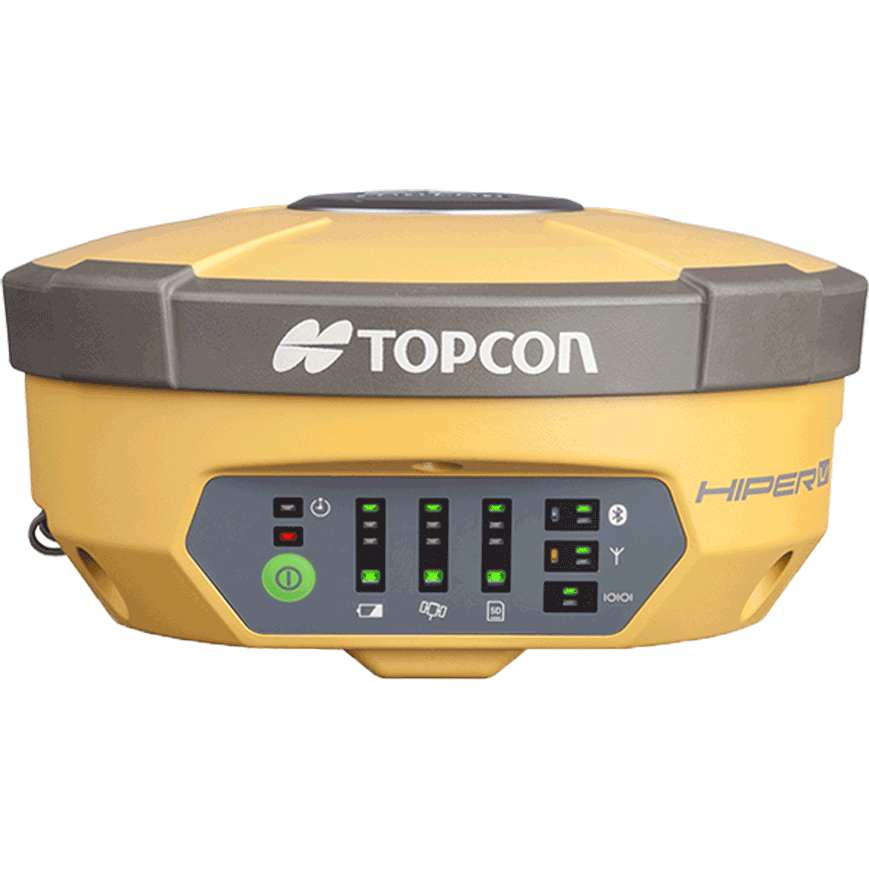
\includegraphics[height=1.4cm]{Chapters/Figures/base_stations/HiPer-V.png} & 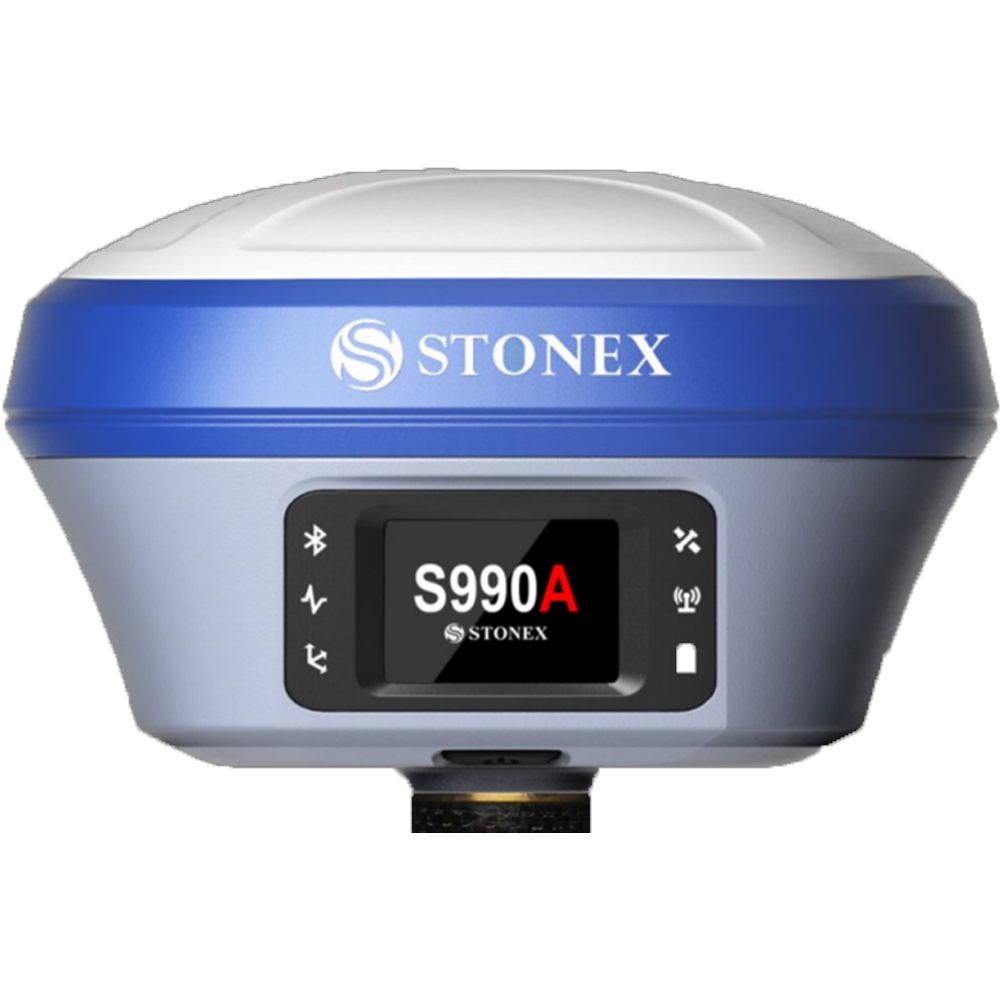
\includegraphics[height=1.4cm]{Chapters/Figures/base_stations/S990A.png}\\
		\bottomrule
	\end{tabular}
\end{table}







% tabela com palavras rodadas:
% \begin{tabular}{m{1em}c}
%     \rotatebox{90}{\textbf{Electrical }}& \makecell{\textbf{Supply} \\ \textbf{Input}\\ \textbf{Battery} \\ \textbf{Autonomy}}\\
% \end{tabular}\\

\newcolumntype{M}[1]{>{\centering\arraybackslash}m{#1}}
\begin{table}[ht]
    \centering
    \captionsetup{justification=centering}
    \caption{Compilation of the most relevant solutions available in the market (as of the date of the present document).}
	\label{tab:currednt_solutions}
    \begin{tabular}{|M{2.5cm}|M{2.5cm}|M{2.5cm}|}
      \hline
      Reconstruction strategy & aa          & bb( \%) \\ \hline
      Classic                 & 3342 voxels & 68 \%   \\ \hline
      VC                      & 4296 voxels & 87 \%   \\ \hline
      V m=7                   & 4745 voxels & 96 \%   \\ \hline
    \end{tabular}
\end{table}

\begin{table}[ht] 
    \centering 
    \begin{tabular}{  >{\raggedright}m{4.5cm}  m{5cm}}      % centered columns (3 columns) 
    \toprule                                   %inserts double horizontal lines 
    Building Block  & Circuits\\  % inserts table heading 
    \midrule\addlinespace[1.5ex]
            Inverting op-amp\\
            (linear amplifier)
            & 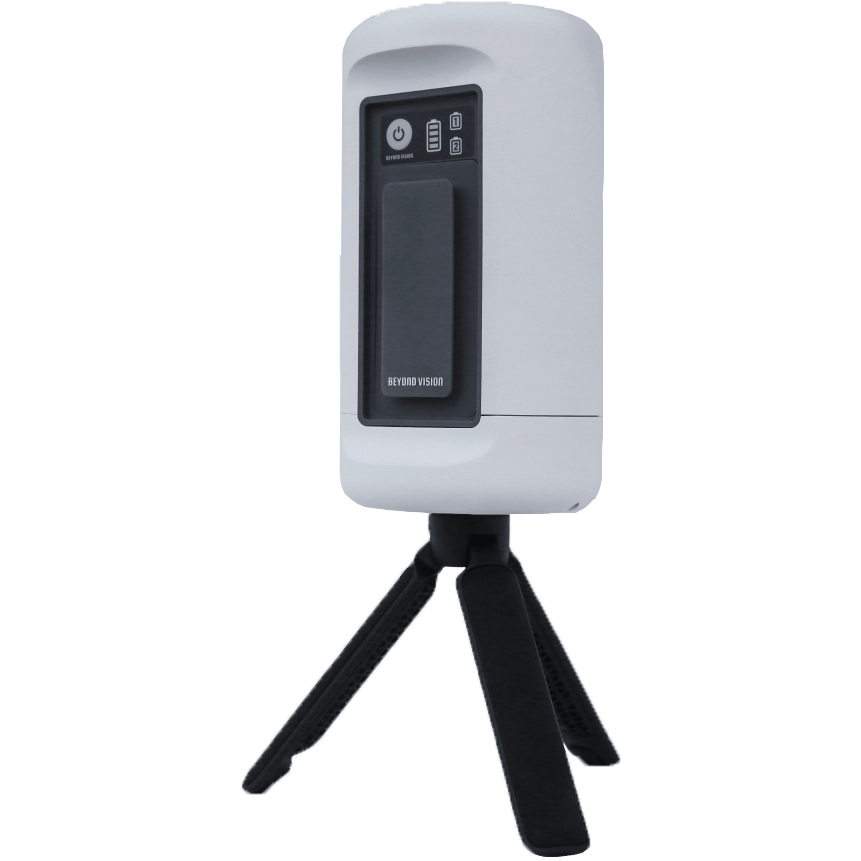
\includegraphics[height=1cm]{Chapters/Figures/base_stations/beRTK_2.png} \\
    \midrule\addlinespace[1.5ex]
            Integrator 
            & 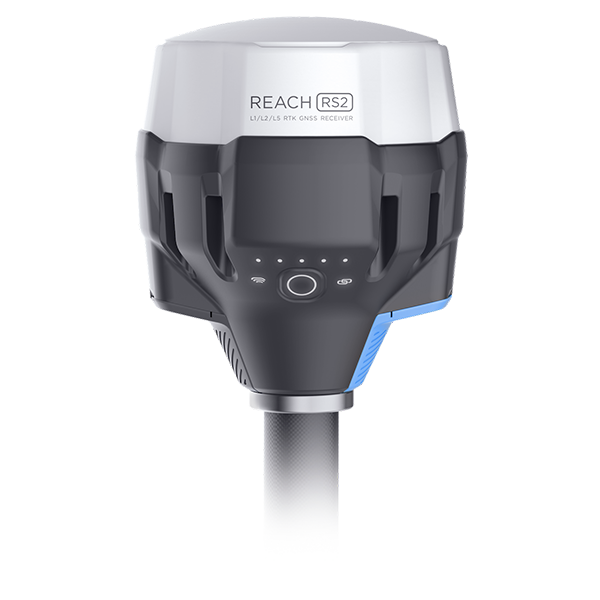
\includegraphics[height=1cm]{Chapters/Figures/base_stations/REACH-RS2.png} \\
    \midrule\addlinespace[1.5ex]
            AC integrator \\ with DC gain
            & 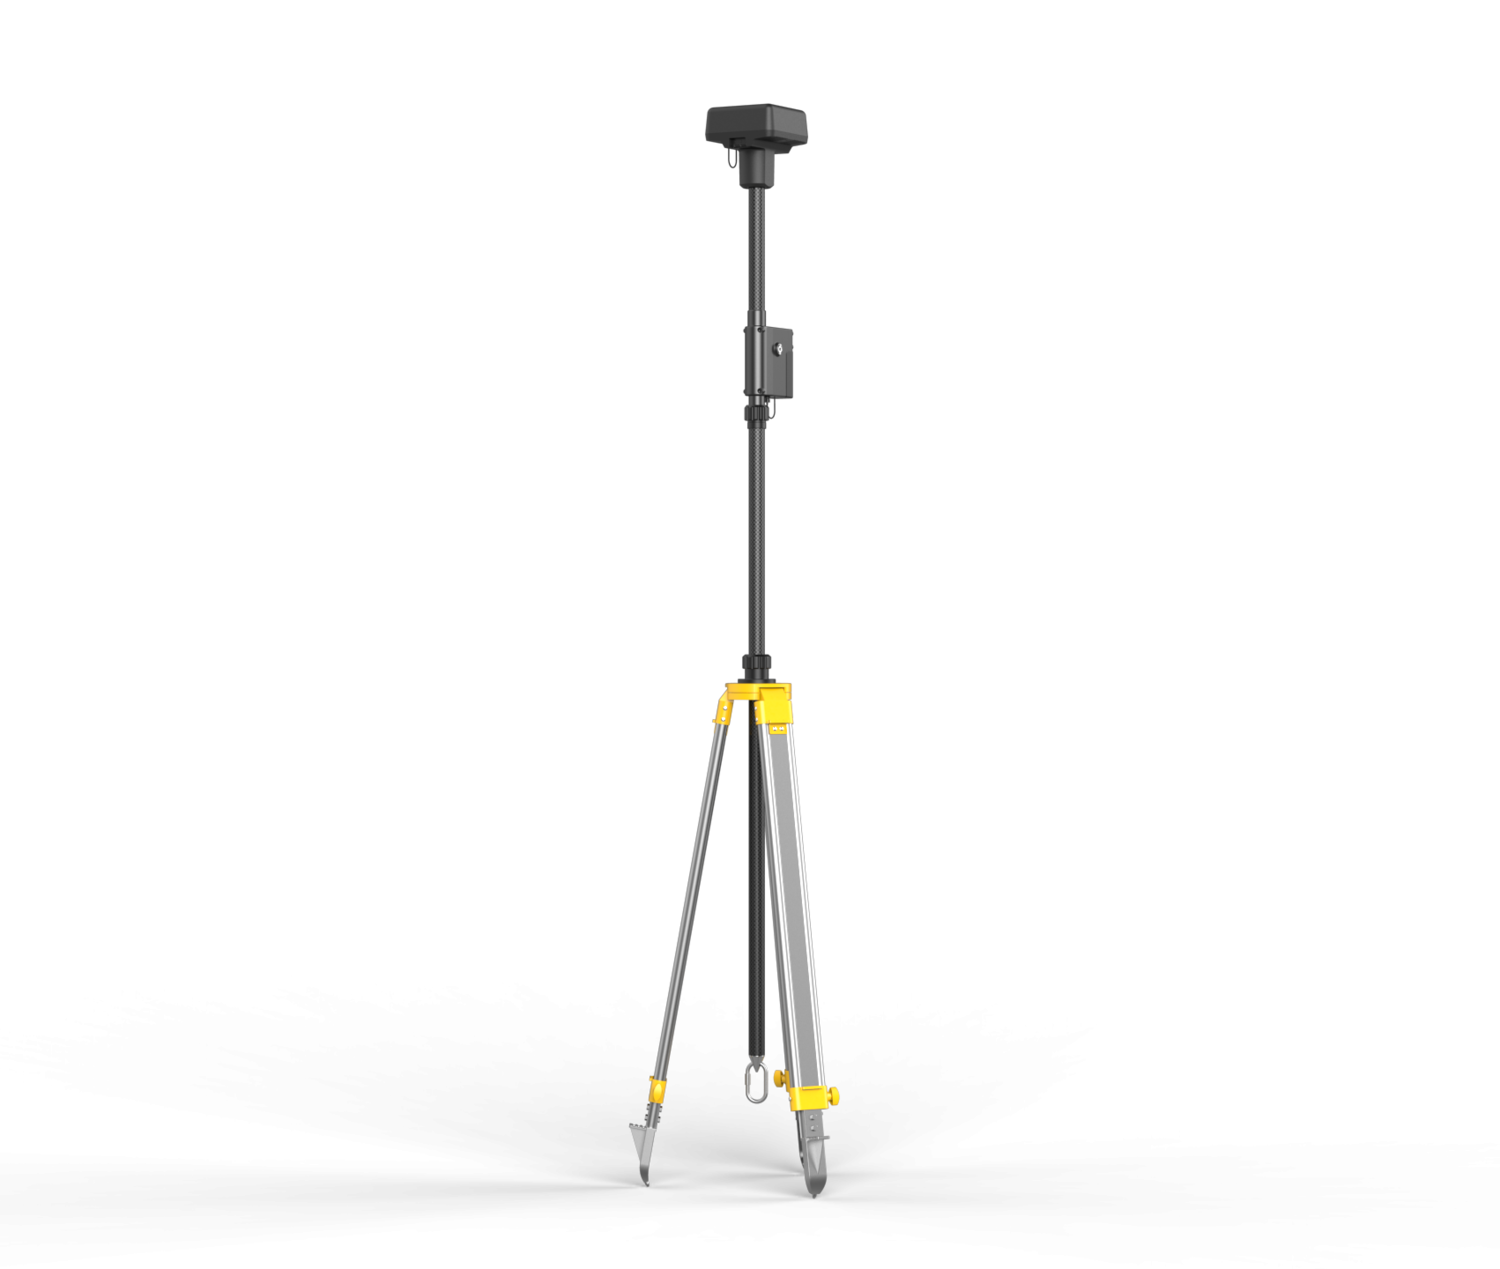
\includegraphics[height=1cm]{Chapters/Figures/base_stations/d-rtk-2.png} \\
    \midrule\addlinespace[1.5ex]
            Differentiator
            & 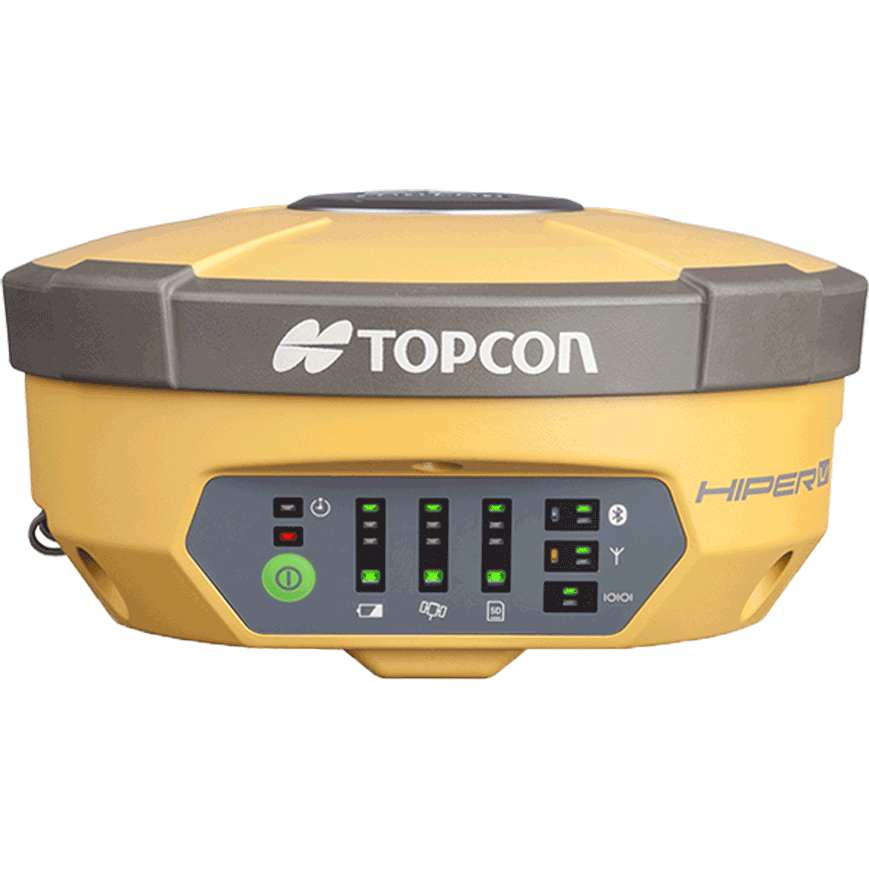
\includegraphics[height=1cm]{Chapters/Figures/base_stations/HiPer-V.png} \\
    \midrule\addlinespace[1.5ex]
            AC differentiator \\ with DC gain
            & 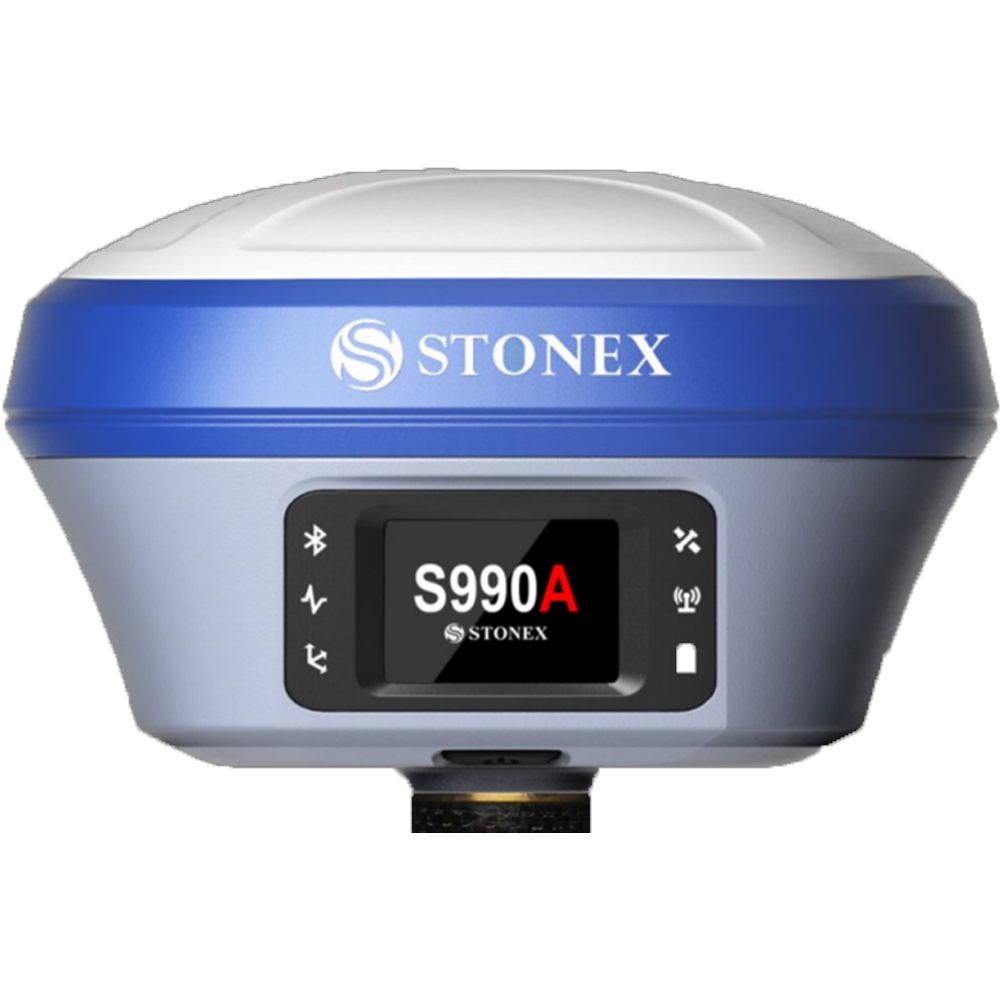
\includegraphics[height=1cm]{Chapters/Figures/base_stations/S990A.png} \\
    \bottomrule
        \end{tabular}
        \caption{A few basic circuit blocks and their frequency response for servo design.}
        \label{table4.2}
\end{table}
